% This example is meant to be compiled with lualatex or xelatex
% The theme itself also supports pdflatex
\PassOptionsToPackage{unicode}{hyperref}
\documentclass[aspectratio=1610, 9pt]{beamer}

% Load packages you need here
\usepackage{polyglossia}
\setmainlanguage{german}

\usepackage{csquotes}
    

\usepackage{amsmath}
\usepackage{amssymb}
\usepackage{mathtools}

\usepackage{hyperref}
\usepackage{bookmark}

% load the theme after all packages

\usetheme[
  showtotalframes, % show total number of frames in the footline
]{tudo}

% Put settings here, like
\unimathsetup{
  math-style=ISO,
  bold-style=ISO,
  nabla=upright,
  partial=upright,
  mathrm=sym,
}

%Titel:
\title{AGN \\(Aktive Galaxienkerne)}
%Autor
\author[N.Breer]{Nils Breer}
%Lehrstuhl/Fakultät
\institute{Fakultät Physik}
%Titelgrafik muss ich einfueren!!!
%\titlegraphic{\includegraphics[width=0.3\textwidth]{content/Bilder/interferenz.jpg}}
\date{28.11.2019}

\begin{document}
\maketitle

\begin{frame}\frametitle{Agenda}
  \begin{itemize}
    \item Eigenschaften von AGN
    \item AGN Modell
    \item Typen von AGN 
    \begin{itemize}
      \item Fanaroff-Riley
      \item Seyfert
      \item GPS
      \item Blazare
    \end{itemize}
    \item Warum sind AGN so interessant?
  \end{itemize}
\end{frame}

\begin{frame}\frametitle{Eigenschaften von AGN}
  \begin{itemize}
    \item AGN bedeutet aktive galactic nucleus
    \item Objekte sind sehr \"ahnlich zu Sternen und kaum zu unterscheiden
    \item Strahlungszentrum ist von der gr\"o\ss e unseres Sonnensystems
    \item Starke Strahlung \"uber gro\ss e Frequenzbereiche von Radiowellen bis Gammastrahlung
  \end{itemize}
\end{frame}

\begin{frame}\frametitle{Eigenschaften von AGN}
  \begin{block}{Energiequelle der starken Leuchtkraft}
    \begin{itemize}
    \item SMBH akkretiert viel Masse, meist Staub und Gaswolken
    \item Impulserhaltung verr\"at, dass Masse nicht direkt ins schwarze Loch fallen kann $\to$ Akkretionsscheibe
    \item Reibungseffekte $\to$ Temperaturerh\"ohung. Teilchen geben Drehimpuls ab und fallen so ins schwarze Loch
    \item Sidenote: normale Galaxien leuchten durch die Sterne, aktive Galaxien leuchten haupts\"achlich durch Kern!
  \end{itemize}
  \end{block}
\end{frame}

\begin{frame}\frametitle{Modell der AGN}
  \begin{columns}
  \begin{column}[c]{0.45\textwidth}
  \begin{itemize}
    \item SMBH mit ca. 100 mio. Sonnenmassen
    \item Akkretions-Scheibe
    \item kolineare Jets (selten auch nur einseitige Jetentwicklung)
    \item broad-line und narrow-line Regionen
    \item Staubtorus
  \end{itemize}
  \end{column}
  \begin{column}[c]{0.45\textwidth}
    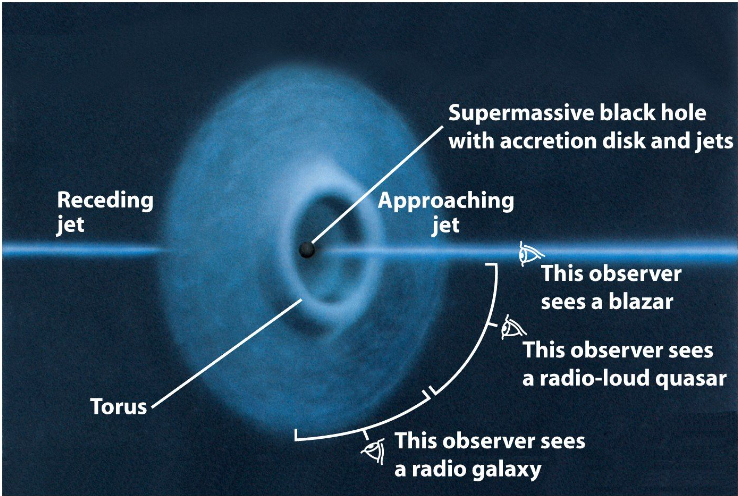
\includegraphics{images/agn-pic.png}
  \end{column}
  \end{columns}
\end{frame}

\begin{frame}\frametitle{Regionen}
  \begin{columns}
  \begin{column}[c]{0.45\textwidth}
    \begin{block}{broad-line (BLR)}
    \begin{itemize}
      \item oberhalb der Akkretionsscheibe
      \item stark ionisierte Wolken $\to$ leuchten der Akkretionsscheibe durch W\"armestrahlung
      \item breite Emissionslinien
    \end{itemize}
    \end{block}
    \end{column}
    \begin{column}[c]{0.45\textwidth}
    \begin{block}{narrow-line (NLR)}
    \begin{itemize}
      \item noch au\ss erhalb der BLR (einige 100 Lichtjahre von der Torus\"offnung entfernt)
      \item stark ionisierte Gas leuchtet
      \item schmale Emissionslinien im Spektrum
    \end{itemize}
    \end{block}
    \end{column}
  \end{columns}
\end{frame}

\begin{frame}\frametitle{Die Akkretionsscheibe}
  \begin{columns}
  \begin{column}[c]{0.45\linewidth}
    \begin{itemize}
      \item um den Torus rotierende Scheibe aus Staub und ionisiertem -bzw. atomarem Gas
      \item Materietransport Richtung Zentrum
    \end{itemize}
  \end{column}
  \begin{column}{0.45\linewidth}
    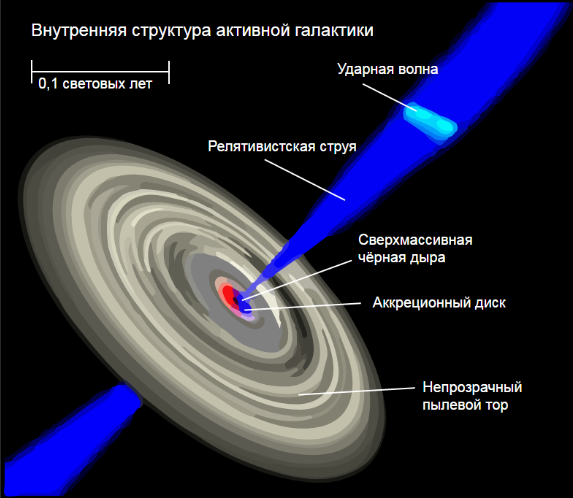
\includegraphics{images/accretion.png}
  \end{column}
  \end{columns}
\end{frame}

\begin{frame}\frametitle{Jets}
  \begin{columns}
  \begin{column}[c]{0.45\linewidth}
    \begin{itemize}
      \item Materiejets senkrecht zur Ebene der Akkretionsscheibe
      \item Geschindigkeiten nahe c
      \item frame-dragging: Effekt, welcher bei sehr massereichen, rotierenden K\"orpern auftritt (verdrillen der Raumzeit in Richtung der Rotation)
      \item $\to$ durch den entstehenden magnetischen Druck wird Materie aus den Polen herausgedr\"uckt
      \item Jets bleiben aber sehr lange kollimiert durch das Magnetfeld
    \end{itemize}
  \end{column}
  \begin{column}{0.45\linewidth}
    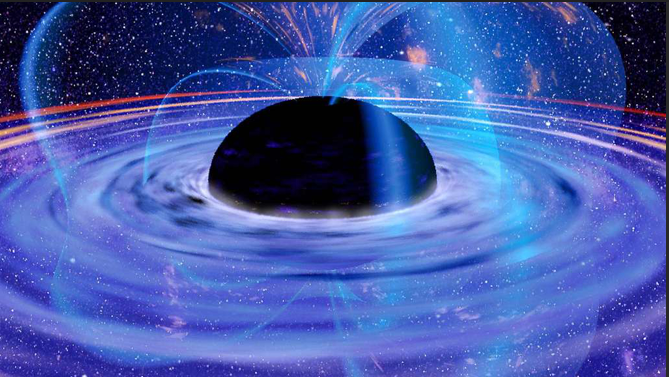
\includegraphics{images/magnetfeld.png}
    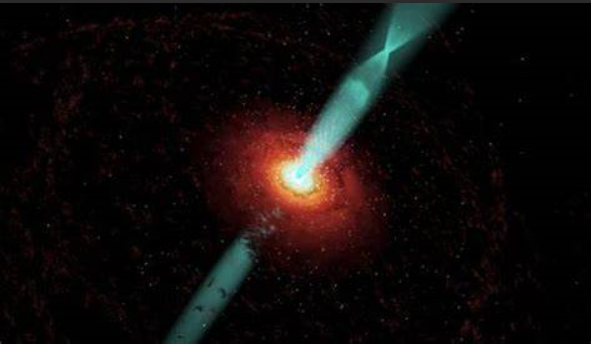
\includegraphics{images/radiojet.png}
  \end{column}
  \end{columns}
\end{frame}

\begin{frame}\frametitle{AGN Typen}
  \begin{block}{3 Typen}
    Die Klassifizierung der AGN "Familie" h\"angt ab von
    \begin{itemize}
      \item dem Beobachtungswinkel
      \item Der Masse des schwarze Lochs
      \item wie viel Masse das schwarze Loch akkretiert
    \end{itemize}
  \end{block}
\end{frame}

\begin{frame}\frametitle{Winkelabh\"angigkeit}
  \begin{block}{Quasi stellar Radio source (Quasar)}
    \begin{itemize}
      \item Objekte mit der weitesten Entfernung (SDSS 1030+0524 ca. 14 mrd. Lichtjahre)
      \item Rotverschiebung $\to$ Entfernungsbestimmung
      \item Detektion durch Radiostrahlung
    \end{itemize}
  \end{block}
\end{frame}

\begin{frame}\frametitle{Seyfert-Galaxien}
  \begin{itemize}
    \item radioleiser Galaxientyp
    \item ca. 90 \% sind Spiralgalaxien
    \item h\"aufigster Galaxientyp mit AGN
    \item Masse des schwarzen Loches kleiner als bei Quasaren
    \item Seyfert 1 und 2 undterscheiden sich darin, ob BLR oder NLR sichtbar sind
  \end{itemize}
\end{frame}

\begin{frame}\frametitle{Fanaroff-Riley Galaxien}
Radiostrahlung meist viel st\"arker als sichtbares Spektrum
  \begin{block}{FR Typ 1}
  \begin{columns}
  \begin{column}{0.45\textwidth}
    \begin{itemize}
      \item Radioemission \~ 1/r
      \item h\"aufig Back-to-Back Jets
    \end{itemize}
  \end{column}
  \begin{column}{0.45\textwidth}
    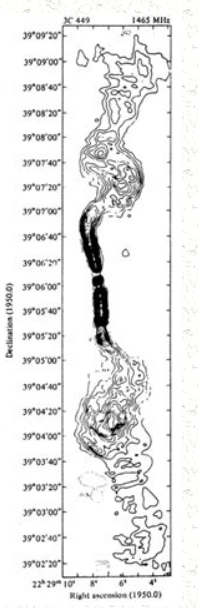
\includegraphics{images/FR1.png}
  \end{column}
  \end{columns}
  \end{block}
\end{frame}

\begin{frame}\frametitle{Fanaroff-Riley Galaxien}
Radiostrahlung meist viel st\"arker als sichtbares Spektrum
  \begin{block}{FR Typ 2}
  \begin{columns}
  \begin{column}[c]{0.45\linewidth}
    \begin{itemize}
      \item Helle "Hot Spots" in sog. Lobes
      \item relativ dunkler Kern
      \item oft einseitiger Jet
      \item i.A. heller als FR-1 durch Keulen
    \end{itemize}
  \end{column}
  \begin{column}[c]{0.45\linewidth}
    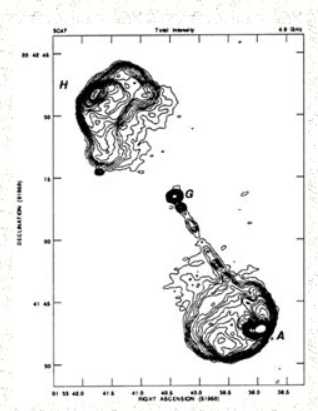
\includegraphics{images/FR2.png}
  \end{column}
  \end{columns}
  \end{block}
\end{frame}

\begin{frame}\frametitle{GPS}
  \begin{itemize}
    \item gigahertz peaked spektrum source
    \item junge (ca. 100 - 1000 jahre alt) Radioquellen mit 1 GHz Strahlung im Maximum
  \end{itemize}
\end{frame}

\begin{frame}\frametitle{Blazare}
  \begin{itemize}
    \item Unterart der AGN und kommmt in 2 Gruppen
    \item OVV (optical violent variable quasars): extrem starke und schnell variierende em-Emission (Radio- bis zu Gammastrahlung)
    \item -> Blickrichtung ziemlich genau in die Jetachse
    \item BL Lacertae Objekte
  \end{itemize}
\end{frame}

\begin{frame}\frametitle{Blazare}
  \begin{block}{BL-Lac Objekte}
  \begin{columns}
  \begin{column}[c]{0.45\linewidth}
    \begin{itemize}
      \item Entdeckung um ca. 1929 (Cuno Hoffmeister) identifiziert als starke Radioquelle um 1968
      \item Blick in Jetachse
      \item Spektrum kontinuirlich (Doppelh\"ocker Spektrum)
      \item bis zu 50 \% der Galaxienmasse in Form von Strahlung
      \item -> Entfernungsbestimmung meist schwierig, da Kern die gesamte Galaxie \"uberstrahlt
    \end{itemize}
    \end{column}
    \begin{column}[c]{0.45\linewidth}
      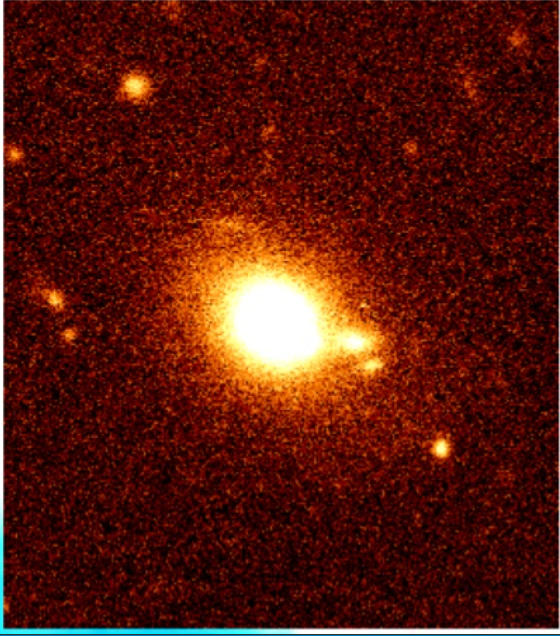
\includegraphics{images/bl-lac-object.png}
    \end{column}
    \end{columns}
  \end{block}
\end{frame}

\begin{frame}\frametitle{Warum sind radiolaute AGN nun interessant?}
  \begin{columns}
  \begin{column}[c]{0.45\textwidth}
  \begin{itemize}
    \item Radiospektren sind auf der Erde gut sichtbar.
    \item Radiowellen werden weniger stark absorbiert von galaktischem Staub als sichtbares Licht
    \item Untersuchung von Pulsaren, SNR, galaktische Zentrum der Milchstra\ss e
    \item Bezugspunkte im Universum
  \end{itemize}
  \end{column}
  \begin{column}[c]{0.45\textwidth}
    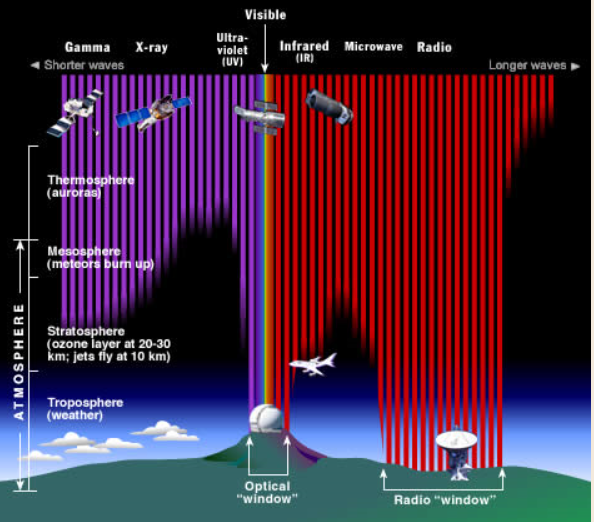
\includegraphics{images/durchlaessigkeit.png}
  \end{column}
  \end{columns}
\end{frame}

\begin{frame}
Quellen: \\
\url{https://www.slideshare.net/antglezatienza/galaxias-activas-87180963} \\
\url{https://ned.ipac.caltech.edu/level5/Urry1/UrryP4_3.html} \\
\url{http://ned.ipac.caltech.edu/level5/Glossary/Essay_fanaroff.html} \\
\url{https://www.astris.info/} \\
\url{https://arxiv.org/pdf/astro-ph/0301332v1.pdf} \\
\url{https://www.nkj.ru/news/29014/}
\end{frame}

\end{document}
